% siunitx and other packages common in papers that Debian only has in
% texlive-latex-extra / texlive-science (from TeX Live in the images, #69),
% with TikZ / pgfplots (texlive-pictures).
\documentclass{article}
\usepackage[T1]{fontenc}
\usepackage{siunitx}
\usepackage{booktabs}
\usepackage{multirow}
\usepackage{makecell}
\usepackage{threeparttable}
\usepackage{enumitem}
\usepackage{wrapfig}
\usepackage{placeins}
\usepackage{nicefrac}
\usepackage{soul}
\usepackage{comment}
\usepackage{inconsolata}
\usepackage{tikz}
\usepackage{pgfplots}
\pgfplotsset{compat=1.18}
\usepackage{algorithm}
\usepackage{algpseudocode}
\usepackage{hyperref}
\usepackage{xurl}
\usepackage{cleveref}
\begin{document}
\section{Results}\label{sec:results}
\SI{9.81}{\metre\per\second\squared}, \qty{3.0e8}{\m\per\s}, \num{12345.678},
\ang{45}, \nicefrac{1}{2}, \hl{highlighted}, \texttt{monospace '0'},
\url{https://example.org/a/very/long/path/that/may/break/anywhere}.
See \cref{sec:results}, \cref{tab:results} and \cref{alg:loop}.
\begin{comment}
This is not typeset.
\end{comment}
\begin{enumerate}[label=(\alph*), noitemsep]
  \item first
  \item second
\end{enumerate}
\begin{table}[h]
  \centering
  \begin{threeparttable}
    \begin{tabular}{l S[table-format=2.1] c}
      \toprule
      \multirow{2}{*}{Model} & {Score} & \makecell{Two\\lines} \\
                             & 12.3    & x                    \\
      \midrule
      B                      & 4.5\tnote{a} & y               \\
      \bottomrule
    \end{tabular}
    \begin{tablenotes}\item[a] A note.\end{tablenotes}
  \end{threeparttable}
  \caption{Results}\label{tab:results}
\end{table}
\FloatBarrier
\begin{algorithm}[h]
  \caption{Loop}\label{alg:loop}
  \begin{algorithmic}[1]
    \For{$i \gets 1$ to $n$}
      \State $s \gets s + i$
    \EndFor
  \end{algorithmic}
\end{algorithm}
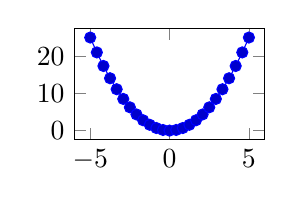
\begin{tikzpicture}
  \begin{axis}[width=4cm, height=3cm]
    \addplot {x^2};
  \end{axis}
\end{tikzpicture}
\end{document}
